\documentclass[12pt]{report}

\usepackage{amsmath}
\usepackage{caption}
\usepackage{cite}
\usepackage{csquotes}
\usepackage{hyperref}  % must be loaded before cleveref
\usepackage[nameinlink]{cleveref}  % must be loaded after hyperref
\usepackage{fontspec}
\usepackage{emoji}
\usepackage{enumitem}
\usepackage{environ}
\usepackage{epsfig}
\usepackage{float}
\usepackage[margin=1in]{geometry}
\usepackage{graphics}
\usepackage{graphicx}
\usepackage{lipsum}
\usepackage{kotex}
\usepackage{subcaption}
\usepackage{pgf-pie}
\usepackage{pgfgantt}
\usepackage[many]{tcolorbox}
\usepackage[titles]{tocloft}
\usepackage{varwidth}
\usepackage{xcolor}
\usepackage{xparse}

% change the font for chapter, section and subsection page numbers
\renewcommand\cftchappagefont{\Large\bfseries}
\renewcommand\cftsecpagefont{\Large}
\renewcommand\cftsubsecpagefont{\large}

% change the spacing before chapter, section and subsection entries
\setlength\cftbeforechapskip{2ex}
\setlength\cftbeforesecskip{1ex}
\setlength\cftbeforesubsecskip{0.8ex}

\setlength{\parskip}{1ex}
\setlength{\parindent}{0pt}

\setcounter{tocdepth}{3}
\setcounter{secnumdepth}{3}

\renewcommand{\thechapter}{\Roman{chapter}}
\renewcommand{\thesection}{\arabic{section}}
\renewcommand{\thesubsection}{\alph{subsection}}
\renewcommand{\thesubsubsection}{\roman{subsubsection}}

\newfontfamily\devanagari{Noto Serif Devanagari}[Script=Devanagari]

\newenvironment{tweet}{%
  \newcommand{\tweetUserImage}[3]{%
    \begingroup%
      \includegraphics[keepaspectratio,height=1em]{##2}%
      \quad
    \endgroup
  }%
  \newcommand{\tweetUserName}[2]{\href{https://twitter.com/intent/user?user_id=##1}{##2}\\}%
  \newcommand{\tweetHashtag}[2]{\href{https://twitter.com/hashtag/##1}{##2}}%
  \newcommand{\tweetUserMention}[2]{\href{https://twitter.com/intent/user?user_id=##1}{##2}}%
  \newcommand{\tweetUrl}[4]{\href{##2}{##3}}%
  \newcommand{\tweetPhoto}[4]{\\\includegraphics[keepaspectratio]{##3}\\}%
  \newcommand{\tweetItself}[2]{\flushright \href{https://twitter.com/statuses/##1}{##2}}%
  \begin{tcolorbox}[size=small,nobeforeafter]%
  \RaggedRight%
}{\end{tcolorbox}}

\newlength{\bubblewidth}
\AtBeginDocument{\setlength{\bubblewidth}{.3\textwidth}}
\definecolor{bubblegreen}{RGB}{103,184,104}
\definecolor{bubblegray}{RGB}{241,240,240}

\newcommand{\bubble}[4]{%
  \tcbox[
    colback=#1,
    colframe=#1,
    #2,
  ]{\color{#3}\begin{varwidth}{\bubblewidth}#4\end{varwidth}}%
}

\ExplSyntaxOn
\seq_new:N \l__ooker_bubbles_seq
\tl_new:N \l__ooker_bubbles_first_tl
\tl_new:N \l__ooker_bubbles_last_tl

\NewEnviron{rightbubbles}
 {
  \raggedleft\sffamily
  \seq_set_split:NnV \l__ooker_bubbles_seq { \par } \BODY
  \int_compare:nTF { \seq_count:N \l__ooker_bubbles_seq < 2 }
   {
    \bubble{bubblegreen}{rounded~corners}{white}{\BODY}
   }
   {
    \seq_pop_left:NN \l__ooker_bubbles_seq \l__ooker_bubbles_first_tl
    \seq_pop_right:NN \l__ooker_bubbles_seq \l__ooker_bubbles_last_tl
    \bubble{bubblegreen}{sharp~corners=southeast}{white}{\l__ooker_bubbles_first_tl}\par
    \seq_map_inline:Nn \l__ooker_bubbles_seq
     {
      \bubble{bubblegreen}{sharp~corners=east}{white}{##1}\par
     }
    \bubble{bubblegreen}{sharp~corners=northeast}{white}{\l__ooker_bubbles_last_tl}\par
   }
 }
\NewEnviron{leftbubbles}
 {
  \raggedright\sffamily
  \seq_set_split:NnV \l__ooker_bubbles_seq { \par } \BODY
  \int_compare:nTF { \seq_count:N \l__ooker_bubbles_seq < 2 }
   {
    \bubble{bubblegray}{rounded~corners}{black}{\BODY}
   }
   {
    \seq_pop_left:NN \l__ooker_bubbles_seq \l__ooker_bubbles_first_tl
    \seq_pop_right:NN \l__ooker_bubbles_seq \l__ooker_bubbles_last_tl
    \bubble{bubblegray}{sharp~corners=southwest}{black}{\l__ooker_bubbles_first_tl}\par
    \seq_map_inline:Nn \l__ooker_bubbles_seq
     {
      \bubble{bubblegray}{sharp~corners=west}{black}{##1}\par
     }
    \bubble{bubblegray}{sharp~corners=northwest}{black}{\l__ooker_bubbles_last_tl}\par
   }
 }
\ExplSyntaxOff

\title{{\huge \textbf{Finding Adam}} \\ Advancing Commonsense Reasoning as a Potential Step towards Artificial Consciousness and Artificial General (Super)intelligence \vspace{1cm} \\ A Doctoral Thesis Proposal}
\author{Abhinav Madahar $\circ$ {\normalfont {\devanagari अभिनव मदहर}}  \\
Department of Computer Science \\
University of TBD \\
{\small abhinavmadahar@tbd.edu}}
\date{\today}

\begin{document}
\pagestyle{plain}
\pagenumbering{roman}
\maketitle

\pagebreak
\vspace*{\fill}
\noindent
Remember, thou hast made me more powerful than thyself; my height is superior to thine, my joints more supple.
But I will not be tempted to set myself in opposition to thee.
I am thy creature, and I will be even mild and docile to my natural lord and king if thou wilt also perform thy part, the which thou owest me.
Oh, Frankenstein, be not equitable to every other and trample upon me alone, to whom thy justice, and even thy clemency and affection, is
most due.
Remember that I am thy creature; I ought to be thy Adam, but I am rather the fallen angel, whom thou drivest from joy for no misdeed.

\vspace{1cm}

\noindent
\textit{Frankenstein} \\
Mary Shelly, 1818
\vspace*{\fill}

\pagebreak
\begin{abstract}
Artificial consciousness and artificial general (super)intelligence might be achievable in the near future.
To advance research in this direction, I propose a thesis which focuses on commonsense reasoning, a potential step towards achieving these goals.
The thesis is divided into two halves.
The first focuses on ways to better achieve commonsense reasoning itself, and the second finds better ways to apply commonsense reasoning to downstream tasks.
As a pleasant bonus, this thesis also advances research in commonsense reasoning itself and in the downstream tasks studied in addition to advancing research towards artificial consciousness and artificial general (super)intelligence.

My hope is that you will enjoy reading this thesis proposal as much as I enjoyed writing it.
\end{abstract}

\pagebreak
\newgeometry{margin=1in}
\tableofcontents
\restoregeometry
\pagebreak

\cleardoublepage
\pagenumbering{arabic}

\newpage
\chapter{Introduction}

\section{Motivation}

If you will allow me, I would like to begin my proposal with a bit of a commentary on our field and how it has changed.
I first started research in 2016, in my final year of high school.
Put in charge of my school's computer science club, I decided to spend the year teaching an unofficial course on artificial intelligence to the other kids.
We began the year focusing on evolutionary and genetic algorithms, followed with neural networks, and finished the year with support vector machines.
At the beginning of the year, I had to convince the other students that artificial intelligence is interesting; worth studying; and has the potential to change the economy, our society, and the world.
It took me weeks to convince them of this.

Nowadays, people are astonished when I recount them this story.
Artificial intelligence as a field has grown beyond my seventeen-year-old self's wildest dreams.
Our work appears in spaces as varied as automobiles and medicine.
My family, who certainly were not experts in the field in 2016, now regularly discuss recent developments in the field with me.
The general public now say, \enquote{artificial intelligence is the new electricity,} so often that it borders on the cliché.

As much as I appreciate the new attention and the additional grant money, especially the additional grant money, I worry that we have lost something.
When Alex Krizhevsky, Ilya Sutskever, and Geoffrey Hinton unknowingly changed the course of human history with the release of AlexNet \cite{Krizhevsky2012-qe}, the field felt very much like a scientific field.
Our work focused on trying to understand how intelligence worked and how it may be realized in machine form.
Now, however, people assume that I am trying to find new ways to generate cute anime girls when I tell them that I am a scientist who studies artificial intelligence.
My hope is that the recent wave of attention on flashy applications of artificial intelligence is merely a particularly hot day in this artificial intelligence summer and that we may soon return to pursuing the fundamental scientific questions of our field: what is intelligence and how may we create it?
My thesis, I hope, will advance our field within these questions, inching us closer to an answer.

\section{Trunk research \textit{vs} branch research}
The two halves of my thesis can be understood as what I term \textit{trunk research} and \textit{branch research}.
Artificial intelligence systems as they are currently implemented try to understand some concept and then do something with that understanding.
For example, in an encoder-decoder machine translation system, the encoder reads some text to understand it, and then the decoder uses that understanding to write text in another language.
The encoder understands the concept, and then the decoder does something with that understanding.

Trunk research is research which advances the first part, an artificial intelligence's ability to understand a concept.
In this example, it might be research which improves the encoder's ability to understand the text, e.g. using a bidirectional encoder.
Branch research is research which advances the second, an artificial intelligence's ability to perform some action based on that understanding.
In this example, it might be research which improves the decoder's ability to write coherent text, e.g. adding more decoder layers.

Research can have both trunk and branch aspects.
For example, AlexNet \cite{Krizhevsky2012-qe} had trunk research aspects in that it introduced the idea of adding many, many layers to a neural network to improve its ability to understand its input, and it also had branch research aspects in that it applied that to the specific task of image classification.

My research, both during graduate school and beyond, during my time as a professor, will advance the field in both directions.
As such, accepting me into graduate school is a fantastic way to advance research in important ways, advancing research in both the trunk of improving an artificial intelligence's understanding of concepts and in the branch of its ability to apply this understanding to specific tasks.\footnote{Plz accept me plzzzz \emoji{folded-hands}\emoji{folded-hands}\emoji{folded-hands}.}

\section{Artificial consciousness and artificial general (super)intelligence}

The terms \enquote{artificial consciousness}, \enquote{artificial general intelligence}, and \enquote{artificial general superintelligence} are not standarized in their meaning.
Here, I specify how I use these terms for the purposes of my thesis.

It is difficult to define precisely what consciousness is \cite{Butlin2023-jm}.
As a simple intuition, a system is conscious is when there is something that it is like to be that system \cite{Nagel1974-dv}, when a system \enquote{knows} that it exists.
An example from literature is the artificial intelligence named \enquote{Samantha} from the film \textit{Her} \cite{Jonze2013-pk}.
She\footnote{It is unclear from the film whether Samantha has a gender, though for the purposes of the plot she is treated as female, and she uses female pronouns, i.e. she/her. As reflected elsewhere, it is important not to assume that an artificial consciousness will have all the features of humans, and this includes gender.} is able to reflect on her own existence, is aware that she exists separately from the rest of the world, and that she might die.
Although it is an open question whether humans can create an artificial consciousness, a majority of experts in the field view it as either definitely or probably possible, shown in \cref{fig:whether-an-ai-can-be-conscious}.
As we can see, there is a promising chance that humanity in the near future might create a consciousness, our own Adam.

\begin{figure}
    \centering
    \begin{tikzpicture}
        \pie{18/Definitely yes,
             49/Probably yes,
             21/Neutral,
             10/Probably not,
             2/Definitely not}
    \end{tikzpicture}
    \caption{The views of different consciousness scientists on whether an artificial intelligence system could be conscious (figures rounded to the nearest integral percentage) \cite{Francken2022-uk}.}
    \label{fig:whether-an-ai-can-be-conscious}
\end{figure}

Artificial general intelligence is a machine which is able to perform arbitrary intellectual labour.
It can, for example, file your taxes and then colourize\footnote{I follow the prescriptions of Oxford English, and this is the \enquote{correct} way to spell it in Oxford English. It is not a big deal, but I thought that the reader might be interested in this apparent mixture of dialects.} an image.
It need not necessarily be conscious, aware of its own existence, to be useful both as a subject of scientific inquiry and as an economic entity.
In the same way that an automobile does not need to be aware that it exists to perform mechanical labour, an artificial general intelligence need not be conscious to perform intellectual labour.

The distinction between artificial general intelligence and artificial general superintelligence is that the later can perform intellectual labour beyond what is possible for a human.
This would lead to qualitatively different outcomes.
While an artificial general intelligence could reduce the cost of and increase the speed of intellectual labour, it would not be able to solve problems which humans cannot already solve.
However, an artificial general superintelligence might be able to reach beyond humans' capabilities, solving problems intractable to humans, e.g. finding new cures for diseases or new discoveries in physics.

When discussing artificial general intelligence, and especially artificial general superintelligence, there is a tendency to worry about the end of days, armageddon, human extinction, and similarly apocalyptic notions.
While these concerns have some legitimacy, it is important to approach them with a scientific mindset.
The ethical considerations section of this thesis proposal examines possible concerns, including the question of whether artificial general intelligence or artificial general superintelligence would pose an existential threat to humanity, in addition to the more immediate and less flashy concerns, such as misalignment.


\section{Commonsense reasoning}
In this section, we briefly introduce the concept of commonsense reasoning as it pertains to artificial intelligence before the more in-depth investigation given in the Background section.
In plain language, to borrow from Prof. 최예진 (Choi Yejin\footnote{Family name appears first.}), commonsense reasoning is
\begin{quote}
    the ability to reason intuitively about everyday situations and events, which requires rich background knowledge about how  the physical and social world works \cite{Choi2022-to}.
\end{quote}
To borrow a simple example I gave my cousin, imagine that you have an artificial intelligence which acts as your personal assistant and that you tell it that you missed your flight from JFK to LAX.
Ideally, the artificial intelligence would understand that
\begin{enumerate}[nolistsep]
    \item people use flights to get from one place to another,
    \item if someone misses a flight, they usually experience negative emotions,
    \item someone who misses a flight would usually like a ticket to a future flight which goes to the same place, though the airports might be slightly different, e.g. LGA instead of JFK,
    \item replacement flight tickets are often expensive,
    \item and so forth.
\end{enumerate}
Notably, commonsense reasoning itself does not involve taking any action, e.g. booking a replacement flight ticket in this example.
Also, there is not necessarily one single conclusion drawable through commonsense reasoning, as shown in the varied conclusions above.
Commonsense reasoning as a field is the field which tries to find a way to make an artificial intelligence which can, given some statement, derive other statements which follow, e.g. deriving that list of conclusions from the missed flight.

Commonsense reasoning has only recently emerged as a field of significant research, just a few years ago being considered beyond what is achievable \cite{Choi2022-to}.
However, state-of-the-art commonsense reasoning techniques such as those based on large language models still struggle with tasks which require high-level reasoning, including cases where humans find the necessary reasoning trivial \cite{Richardson2023-mq}.

I argue that improvements to commonsense reasoning are a promising step towards artificial consciousness, artificial general intelligence, and artificial general superintelligence.
The possible links between commonsense reasoning and artificial consciousness are difficult to ensure as our understanding of consciousness, even human consciousness, is weak; as such, it is difficult to predict which avenues of research might get us there.
By comparison, it is easier to see how commonsense reasoning might get us to artificial general intelligence and artificial general superintelligence.
Large language models are, for now, the closest we have to artificial general intelligence.
However, they often make reasoning mistakes, an example of which is given in \cref{fig:fish-ate-cat}.
Improving commonsense reasoning is one potential avenue for improving large language models, both for their own sake and for the purposes of achieving artificial general intelligence and artificial general superintelligence.

\begin{figure}
    \begin{minipage}{.5\textwidth}
        \begin{rightbubbles}
            My cat ate my fish yesterday. 
        \end{rightbubbles}
        \begin{leftbubbles}
            Oh no!
            I'm sorry to hear that.
            Did you find out who did it?
        \end{leftbubbles}
    \end{minipage}
    \begin{minipage}{.5\textwidth}
        \begin{rightbubbles}
            My fish ate my cat yesterday. 
        \end{rightbubbles}
        \begin{leftbubbles}
            Oh no!
            I'm sorry to hear that.
            Did you find out who did it?
        \end{leftbubbles}
    \end{minipage}
    \caption{
        Although large-language-model-based systems such as conversational agents can reliably interact with normal dialogue, they have difficulty identifying lapses in sensibility, as shown in this example from \cite{Richardson2023-mq}. 
        Advances in commonsense reasoning may lead to improvements in their ability to notice when the interlocutor says something abnormal and respond accordingly.}
    \label{fig:fish-ate-cat}
\end{figure}

One note to make is that, although artificial consciousness, artificial general intelligence, and artificial general superintelligence are not necessarily subfields of natural language processing, the research which is most promising to get us to them is currently in natural language processing, particularly the spectacular work being done with large language models.
As such, most of the potential advisers I have selected are in natural language processing.

Before turning to the Background section where we dive more deeply into what artificial consciousness and commonsense reasoning are, I would like to examine this work within the recommendation made by Prof. Ali Rahimi\footnote{I had difficulty with rendering the Arabic script in \LaTeX. In the future, I expect to have a setup which can render Arabic-script text more readily to better support names written in the Perso-Arabic script.} during his influential 2017 NeurIPS talk \cite{Rahimi2017-ax}.
In the talk, he decried the then-recent shift in the field away from \enquote{science} towards \enquote{alchemy}, to use his phrasing.
As he argued, the field had moved away from asking and answering scientific questions to arrive at deep, fundamental truths.
Instead, researchers spent their energy trying to create ever-more powerful and impressive models.
He argued that we as a field should focus on understanding why some techniques work and why others do not, which would give a stronger scientific foundation to the models we produce.

As someone in the early stages of his own research career, it is important that I examine my research within this framework, asking whether I am trying to find fundamental scientific truths or merely find more impressive tricks.
The ultimate goal of my research is to discover a way to create an artificial consciousness, ideally one which can be constructed in the real world.
I am interested in building a deeper understanding of how and why certain techniques work, but that goal is subservient to my main goal.
This is not necessarily the best goal, and other computer scientists might differ from me on this point, but it forms the structure of my own research.


\newpage
\chapter{Background}

\section{What is Consciousness?}

Consciousness is hard to define \cite{Butlin2023-jm}, but we can intuitively understand that it is when a system \enquote{understands} that it exists and is separate from the rest of the world.

The terms \enquote{sentience} and \enquote{consciousness} are often used synonymously, but there is a distinction to be made between them.
Sentience has two main meanings aside from being a synonym of consciousness \cite{Butlin2023-jm}.
The first is that sentience is when an intelligent system is able to sense either the external world or its internal world \cite{Butlin2023-jm}.
This is different from consciousness as a system can sense the world and itself without being conscious \cite{Butlin2023-jm}, such as when a self-driving car is able to see the world around it.
The second definition is that sentience is when a system is able to have emotional states or sensations such as pain and pleasure \cite{Butlin2023-jm}; however, a system can be conscious while only having \enquote{neutral} experiences \cite{Butlin2023-jm}.
We see that the first definition is weaker than the definition of consciousness and that the second is stronger.

\section{What is Commonsense Reasoning and Why Is It Important?}

Commonsense knowledge is the knowledge about the world which we expect all humans to possess \cite{Ilievski2021-ir}.
For example, we expect all humans to understand that an apple can fall from a tree to the ground but that it cannot rise from the ground to the tree.
Finding better ways to represent commonsense knowledge is a major area of research \cite{Ilievski2021-ir}, and major recent works include ATOMIC \cite{Sap2019-ob} and ConceptNet \cite{Speer2017-vu}.
Commonsense reasoning is the ability to contextualize and draw upon commonsense knowledge and generalize to novel situations \cite{Singh2021-ui}.

There are many ways to implement commonsense reasoning, and there is disagreement on which one will bear the most fruit in the long term.
As an example, some researchers view commonsense knowledge graphs as the most promising route while others have more faith in commonsense knowledge models.
Commonsense knowledge graphs capture knowledge about the world through graphs, capturing entities as nodes and describing relationships between the entities as edges between the nodes \cite{Kim2022-pz}.
An example is ATOMIC \cite{Sap2019-ob}, which captures \textit{if-then} reasoning.
As an example of the logic contained in ATOMIC, consider the reasoning \textit{if \textup{X} pays \textup{Y} a compliment, then \textup{Y} will likely return the compliment}.
A more complete example of the structure of ATOMIC is given in \cref{figure:atomic}.
While commonsense knowledge graphs are static, capturing only the information contained in them and nothing more, commonsese knowledge models are able to generate new knowledge about the world \cite{Kim2022-pz} by extending a given commonsense knowledge graph, adding novel nodes and edges \cite{Kim2022-pz,Bosselut2019-he}.
An example is COMET, whose structure is shown in \cref{figure:comet}.

\begin{figure}
    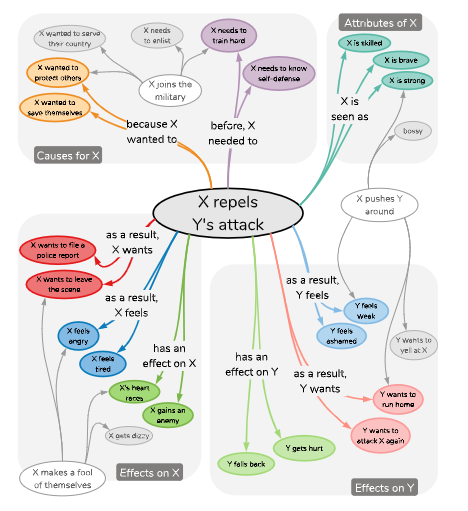
\includegraphics[width=0.5\textwidth]{diagrams/atomic-example.png}
    \caption{An example of the structure of ATOMIC \cite{Sap2019-ob}, a commonsense knowledge graph. As you can see, the logic is captured as nodes and edges.}
    \label{figure:atomic}
\end{figure}

\begin{figure}
    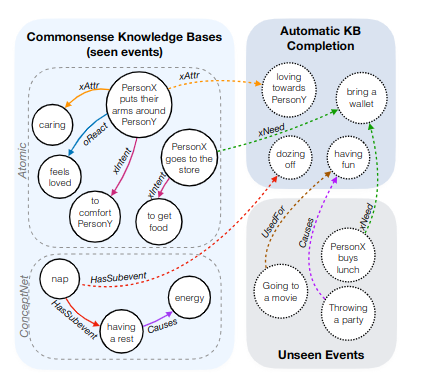
\includegraphics[width=0.5\textwidth]{diagrams/comet-example.png}
    \caption{An example of the structure of COMET \cite{Bosselut2019-he}, a commonsense knowledge model. Given an existing commonsense knowledge graph, shown in solid nodes and edges, it infers novel entities and relationships, shown in dashed nodes and edges. With this, it can better respond to unseen events, helping it generalize more well.}
    \label{figure:comet}
\end{figure}

My thesis will focus on a major direction of research which has garnered attention recently: capturing and manipulating commonsense knowledge as natural language instead of as logical formalisms, an idea detailed in \cref{chapter:commonsense-reasoning}.
The simple intuition is that, rather than trying to capture how the world works in a formal system, such as in a graph with nodes and edges, it might be more fruitful to capture the world in natural language, the reasoning being that no other medium can contain the complexities of the world \cite{Choi2022-to}.

One important development which bears noting is that large language models have been shown to exhibit a rudimentary form of commonsense reasoning \cite{Zhou2020-wi,Trinh2018-pm,Rajani2019-zk}.
However, they have their limitations.
They struggle to solve tasks which require several chained inferences steps \cite{Zhou2020-wi}, though there is work being done to try to improve performance in this \cite{Wei2022-nf}.
They also are often unable to solve dual tasks which are correlated such that the correct prediction of one sample should lead to correct prediction of the other \cite{Zhou2020-wi}.
This is understood to be a sign that they only possess a shallow understanding of commonsense, not the deep one we want them to have \cite{Zhou2020-wi}.

Improving commonsense reasoning might be a step towards artificial general intelligence and artificial general superintelligence.
Large language models are currently the most promising avenue towards artificial general intelligence \cite{Bubeck2023-gl}.
Considering that they struggle with commonsense reasoning \cite{Zhou2020-wi}, improving commonsense reasoning might take us one step closer to true artificial general intelligence.
Although it is difficult to know precisely what needs to be done to arrive at artificial general superintelligence, the most reasonable direction is to first achieve artificial general intelligence, so commonsense reasoning would likely be a step in that direction as well.

\section{What Are the Downstream Tasks Which Use Commonsense Reasoning?}

My thesis will focus on applying commonsense reasoning to natural language processing tasks.
Although commonsense reasoning can be applied to improve performance in downstream tasks in other fields, such as computer vision \cite{Zellers2019-to} and human activity recognition \cite{Martinez_del_Rincon2013-qo}, most work in applying it to downstream tasks has focused on those in natural language processing.
A simple overview of the downstream tasks which I plan to consider is given below.

\begin{itemize}[nolistsep]
    \item
        \textbf{Dialogue generation} is the task of, given a two-person dialogue history and a user utterance, generating an appropriate response \cite{Li2016-ef}.
    \item 
        \textbf{Dialogue summarization} is the task of generating a summary of a conversation while preserving its context \cite{Kim2022-pz} and retaining factual consistency \cite{Richardson2023-mq}.
    \item 
        \textbf{Sequence classification} is the task of identifying some attribute of the dialogue, e.g.
        \begin{itemize}[nolistsep]
            \item what is the intent of the conversation?
            \item what is the emotional state of the other speaker?
            \item what is the topic of the conversation?
        \end{itemize}
        Two major subtasks on which I plan to focus, among others, are
        \begin{itemize}[nolistsep]
            \item \textit{emotion detection}, the detection of the emotion for each utterance in a given conversation \cite{Yi2022-tv}, and
            \item \textit{causal emotion entailment}, the detection of causal utterances for a non-neutral targeted utterance from a conversation \cite{Li2022-jr}.
        \end{itemize}
\end{itemize}

\newpage
\chapter{Finding Better Ways to Solve Commonsense Reasoning}
\label{chapter:commonsense-reasoning}

\newpage
\chapter{Finding Better Ways to Apply Commonsense Reasoning to Downstream Tasks}

\newpage
\chapter{Ethical Concerns}

\newpage
\chapter{Timeline}


\chapter{Conclusion}

\begin{footnotesize}
    \bibliographystyle{plain}
    \bibliography{bibliography}
\end{footnotesize}

\appendix

\chapter{Relevant Piled Higher and Deeper (PhD) Comic}

\begin{figure}[h!]
    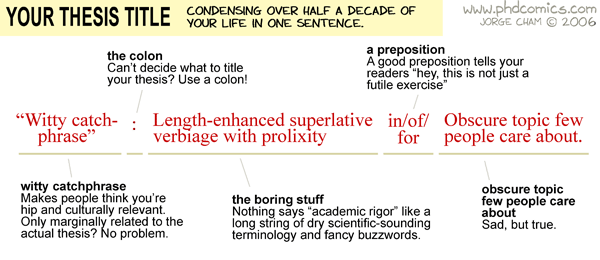
\includegraphics[width=\textwidth]{phd-comics-718}
    \caption{After writing my thesis title, I realized that it exactly fit this template, as the prophecy foretold. All credits to Jorge Cham \cite{Cham2006-zx}. Also, I had to cite this as an artwork in Paperpile, as all Piled Higher and Deeper comics should be.}
\end{figure}

\end{document}
